% Options for packages loaded elsewhere
\PassOptionsToPackage{unicode}{hyperref}
\PassOptionsToPackage{hyphens}{url}
%
\documentclass[
]{article}
\usepackage{amsmath,amssymb}
\usepackage{iftex}
\ifPDFTeX
  \usepackage[T1]{fontenc}
  \usepackage[utf8]{inputenc}
  \usepackage{textcomp} % provide euro and other symbols
\else % if luatex or xetex
  \usepackage{unicode-math} % this also loads fontspec
  \defaultfontfeatures{Scale=MatchLowercase}
  \defaultfontfeatures[\rmfamily]{Ligatures=TeX,Scale=1}
\fi
\usepackage{lmodern}
\ifPDFTeX\else
  % xetex/luatex font selection
\fi
% Use upquote if available, for straight quotes in verbatim environments
\IfFileExists{upquote.sty}{\usepackage{upquote}}{}
\IfFileExists{microtype.sty}{% use microtype if available
  \usepackage[]{microtype}
  \UseMicrotypeSet[protrusion]{basicmath} % disable protrusion for tt fonts
}{}
\makeatletter
\@ifundefined{KOMAClassName}{% if non-KOMA class
  \IfFileExists{parskip.sty}{%
    \usepackage{parskip}
  }{% else
    \setlength{\parindent}{0pt}
    \setlength{\parskip}{6pt plus 2pt minus 1pt}}
}{% if KOMA class
  \KOMAoptions{parskip=half}}
\makeatother
\usepackage{xcolor}
\usepackage[margin=1in]{geometry}
\usepackage{longtable,booktabs,array}
\usepackage{calc} % for calculating minipage widths
% Correct order of tables after \paragraph or \subparagraph
\usepackage{etoolbox}
\makeatletter
\patchcmd\longtable{\par}{\if@noskipsec\mbox{}\fi\par}{}{}
\makeatother
% Allow footnotes in longtable head/foot
\IfFileExists{footnotehyper.sty}{\usepackage{footnotehyper}}{\usepackage{footnote}}
\makesavenoteenv{longtable}
\usepackage{graphicx}
\makeatletter
\def\maxwidth{\ifdim\Gin@nat@width>\linewidth\linewidth\else\Gin@nat@width\fi}
\def\maxheight{\ifdim\Gin@nat@height>\textheight\textheight\else\Gin@nat@height\fi}
\makeatother
% Scale images if necessary, so that they will not overflow the page
% margins by default, and it is still possible to overwrite the defaults
% using explicit options in \includegraphics[width, height, ...]{}
\setkeys{Gin}{width=\maxwidth,height=\maxheight,keepaspectratio}
% Set default figure placement to htbp
\makeatletter
\def\fps@figure{htbp}
\makeatother
\setlength{\emergencystretch}{3em} % prevent overfull lines
\providecommand{\tightlist}{%
  \setlength{\itemsep}{0pt}\setlength{\parskip}{0pt}}
\setcounter{secnumdepth}{5}
\newlength{\cslhangindent}
\setlength{\cslhangindent}{1.5em}
\newlength{\csllabelwidth}
\setlength{\csllabelwidth}{3em}
\newlength{\cslentryspacingunit} % times entry-spacing
\setlength{\cslentryspacingunit}{\parskip}
\newenvironment{CSLReferences}[2] % #1 hanging-ident, #2 entry spacing
 {% don't indent paragraphs
  \setlength{\parindent}{0pt}
  % turn on hanging indent if param 1 is 1
  \ifodd #1
  \let\oldpar\par
  \def\par{\hangindent=\cslhangindent\oldpar}
  \fi
  % set entry spacing
  \setlength{\parskip}{#2\cslentryspacingunit}
 }%
 {}
\usepackage{calc}
\newcommand{\CSLBlock}[1]{#1\hfill\break}
\newcommand{\CSLLeftMargin}[1]{\parbox[t]{\csllabelwidth}{#1}}
\newcommand{\CSLRightInline}[1]{\parbox[t]{\linewidth - \csllabelwidth}{#1}\break}
\newcommand{\CSLIndent}[1]{\hspace{\cslhangindent}#1}
\usepackage{setspace}\linespread{1.25}
\usepackage[fontsize=12pt]{scrextend}
\usepackage[left]{lineno}
\usepackage[labelformat=empty]{caption}
\usepackage{longtable}
\usepackage{booktabs}
\ifLuaTeX
  \usepackage{selnolig}  % disable illegal ligatures
\fi
\IfFileExists{bookmark.sty}{\usepackage{bookmark}}{\usepackage{hyperref}}
\IfFileExists{xurl.sty}{\usepackage{xurl}}{} % add URL line breaks if available
\urlstyle{same}
\hypersetup{
  hidelinks,
  pdfcreator={LaTeX via pandoc}}

\author{}
\date{\vspace{-2.5em}}

\begin{document}

\textbf{N-Methyl-D-aspartate receptor hypofunction causes recurrent and
transient failures of perceptual inference}\\
\strut \\

\textbf{Authors}:

Veith Weilnhammer\(^{1,2, 3,ec}\), Marcus Rothkirch\(^{1, 4, ec}\),
Deniz Yilmaz\(^{1,5,6,7, ec}\), Merve Fritsch\(^{1}\), Lena Esther
Ptasczynski\(^{1,5}\), Katrin Reichenbach\(^{1}\), Lukas
Rödiger\(^{1}\), Philip Corlett\(^{8}\), Philipp Sterzer\(^{9}\)\\
\strut \\
\textbf{Affiliations}:

\(^{1}\) Department of Psychiatry, Charité-Universitätsmedizin Berlin,
corporate member of Freie Universität Berlin and Humboldt-Universität zu
Berlin, Germany\\
\(^{2}\) Berlin Institute of Health, Charité-Universitätsmedizin Berlin
and Max Delbrück Center, Germany\\
\(^{3}\) Helen Wills Neuroscience Institute, University of California
Berkeley, USA\\
\(^{4}\) Medical School Berlin, Hochschule für Gesundheit und Medizin,
Germany\\
\(^{5}\) Berlin School of Mind and Brain, Humboldt-Universität zu
Berlin, Germany\\
\(^{6}\) Max Planck School of Cognition, Leipzig, Germany\\
\(^{7}\) Department of Psychiatry and Psychotherapy, LMU University
Hospital, Munich, Germany\\
\(^{8}\) Department of Psychiatry, Yale University School of Medicine,
New Haven, USA\\
\(^{9}\) Department of Psychiatry (UPK), University of Basel,
Switzerland\\
\strut \\
\textbf{Contributions}:

\(^{ec}\) Equal contribution\\
\strut \\
\textbf{Corresponding Author}:

Veith Weilnhammer, Helen Wills Neuroscience Institute, University of
California Berkeley, USA, email:
\href{mailto:veith.weilnhammer@gmail.com}{\nolinkurl{veith.weilnhammer@gmail.com}}\\

\newpage

\linenumbers

\hypertarget{abstract}{%
\section{Abstract}\label{abstract}}

Perception is known to alternate between an external mode, driven by sensory inputs, and an internal mode, shaped by prior knowledge about the world. Using a double-blind, placebo-controlled, cross-over experiment in healthy human participants, we investigated the effects of the N-Methyl-D-aspartate receptor (NMDAR) antagonist S-ketamine on the alternation between external and internal modes. We found that pharmacologically induced NMDAR hypofunction causes a shift of perception toward the external mode. Similarly, a case-control study revealed that individuals with paranoid schizophrenia, a disorder repeatedly associated with NMDAR hypofunction, spend more time in the external mode. This NMDAR-dependent increase in the external mode suggests that the symptoms of schizophrenia are caused by recurring dissociations of perception from prior knowledge about the world.

\hypertarget{main}{%
\section{Main}\label{main}}

Imagine a dimly lit room at a crowded party, where unclear visual
signals, indistinct sounds, and complex social interactions allow for
multiple - and sometimes false - interpretations. In such ambiguity,
failures of perceptual inference, the ability to contextualize sensory
inputs with prior knowledge about the world, can lead to profound
departures from reality: Faces obscured in shadow may appear distorted,
random noise could be perceived as a whisper, and friendly smiles might
seem derogatory.

This example illustrates why a disruption of perceptual inference is
likely to play a crucial role in schizophrenia (Scz), a chronic and
severe mental disorder characterized by psychotic symptoms such as
delusions and hallucinations\textsuperscript{1--3}. Yet despite
considerable progress in the computational understanding of psychosis,
two key questions have remained unanswered.

The first question concerns the neural mechanisms that cause perceptual
inference to fail in Scz. Several lines of evidence point to
N-Methyl-D-aspartate receptor (NMDAR) hypofunction as a key factor in
the pathophysiology of psychosis\textsuperscript{4}. NMDAR
antibodies\textsuperscript{5} and antagonists such as
ketamine\textsuperscript{6} mimic the symptoms of Scz, which is itself
associated with a reduction of NMDAR density in prefrontal
cortex\textsuperscript{7}. NMDARs control the ratio of neural excitation
and inhibition\textsuperscript{8}, block the release of midbrain
dopamine\textsuperscript{9}, enable cortical
feedback\textsuperscript{10} and support synaptic short term
plasticity\textsuperscript{11}. While these NMDAR-dependent mechanisms
are likely critical for perceptual inference, it is yet to be determined
how NMDAR hypofunction may cause the psychotic symptoms that
characterize Scz.

The second unresolved question concerns the temporal dynamics of
psychotic experiences, which often unfold as short-lived events spanning
from seconds to minutes, especially at early stages of
Scz\textsuperscript{12,13}. The transient nature of psychotic
experiences challenges models that assume a constant disruption of
perceptual inference\textsuperscript{1--3}. A solution to this problem
is suggested by the recent observation that perceptual inference is
subject to spontaneous fluctuations over time that occur at a timescale
compatible with the duration of individual psychotic
experiences\textsuperscript{14--16}. Such fluctuations have been related
to two opposing modes of inference, during which perception is driven
predominantly either by external inputs or by internal predictions that
stem from recent perceptual experiences\textsuperscript{17} (Figure 1A).
Although preliminary evidence indicates a tendency toward the external
mode in people with Scz\textsuperscript{18}, the neural mechanisms of
mode fluctuations and their potential implications in psychosis have
remained elusive.

The objective of the current study was therefore twofold: First, to test
whether NMDAR hypofunction causes changes in perceptual inference that
characterize Scz; and second, to explore the effect of NMDAR
hypofunction on ongoing fluctuations in perceptual inference that may
explain the transient nature of psychotic experiences. We addressed
these aims in a double-blind placebo-controlled cross-over experiment in
28 healthy human participants. The participants attended two
experimental sessions during which they received a continuous
intravenous infusion of either the NMDAR antagonist S-ketamine at a dose
of 0.1 mg/kg/h or a saline placebo. In each session, the participants
viewed ten 120 sec blocks of an ambiguous structure-from-motion (SFM)
stimulus that induced the experience of a sphere rotating around a
vertical axis, and reported changes in the perceived direction of
rotation (leftward vs.~rightward movement of the front surface) as well
as their confidence in the choice (Figure 1B and Supplemental Video S1).

The ambiguity of the display induced the phenomenon of bistable
perception, where spontaneous changes in the perceived direction of
rotation occurred in average intervals of \(13.75\) ± \(3.09\) sec.~In
line with previous results\textsuperscript{19,20}, these changes in
perception occurred with a probability of \(0.11\) ±
\(\ensuremath{8.67\times 10^{-3}}\) at brief depth-symmetric
configurations of the stimulus (see Supplemental Video S1 and
Supplemental Figure S1A). We therefore divided the continuous behavioral
reports into a sequence of discrete states \(t\). Each state was
associated with a perceptual experience \(y_t\), confidence \(c_t\) and
the external input \(s_t\).

Bistable perception can be conceptualized as an inferential process
about the cause of \(s_t\), in which previous experiences (\(y_{t-1}\))
reflect internal predictions that provide prior knowledge about the
interpretation \(y_t\) of the ambiguous stimulus\textsuperscript{20}
(Figure 1C). To test how NMDAR antagonism altered the balance between
external inputs and internal predictions, we attached a 3D signal to a
fraction of the stimulus dots. The signal-to-ambiguity ratio (SAR)
ranged from complete ambiguity to full disambiguation across five levels
and remained constant in each block of the experiment. By changing the
direction of rotation enforced by the 3D signal at random in average
intervals of 10 sec, we created dynamic conflicts between the
SAR-weighted input \(s_t\) and the stabilizing internal prediction
\(y_{t-1}\). As expected, we found that \(y_t\) was driven by both
\(s_t\) (\(\beta_S\) = \(3.01\) ± \(0.06\)) and \(y_{t-1}\) (\(\beta_P\)
= \(2.06\) ± \(0.03\)). Importantly, S-ketamine caused perception to
shift toward \(s_t\) (\(0.45\) ± \(0.08\), z = \(5.6\), p =
\(\ensuremath{1.71\times 10^{-7}}\); Figure 2A and Supplemental Figure
S2), indicating a stronger weighting of external inputs over internal
predictions during pharmacologically induced NMDAR hypofunction.

Next, we performed the same analysis on data from a previous
case-control study using an analogous task in patients with
Scz\textsuperscript{19}. In Scz patients and controls, \(y_t\) was
influenced by the SAR-weighted input \(s_t\) (\(\beta_S\) = \(2.77\) ±
\(0.11\)) and the stabilizing prediction \(y_{t-1}\) (\(\beta_{P}\) =
\(1.5\) ± \(0.03\)). Similar to S-ketamine, \(s_t\) had a larger impact
on perception in Scz patients than controls (\(0.75\) ± \(0.15\), z =
\(4.96\), p = \(\ensuremath{5.6\times 10^{-6}}\); Figure 2E and
Supplemental Figure S3). Together, these results align with the
canonical predictive processing theory of Scz\textsuperscript{1--3}:
Pharmacologically-induced NMDAR hypofunction and Scz are associated with
a shift of perceptual inference toward external inputs, and away from
stabilizing internal predictions. NMDAR hypofunction may thus trigger
psychotic experiences by causing erratic inferences about ambiguous
sensory information.

As a mechanism for symptoms that are transient and recurring,
NMDAR-dependent changes in perceptual inference should not be constant,
but fluctuate dynamically at a timescale that is compatible with the
duration of individual psychotic experiences. We tested this prediction
in Hidden Markov Models (HMM) that inferred transitions between two
latent states, each linked to an independent general linear model (GLM)
that predicted \(y_t\) from \(s_t\) and \(y_{t-1}\). The \(\beta\)
weights quantified the sensitivity to ambiguous sensory information
(\(\beta_S \times s_t\)) relative to the stabilizing effect of internal
predictions provided by preceding experiences
(\(\beta_{P} \times y_{t-1}\)), and allowed us to evaluate dynamic
changes in the balance \(\Delta_{S-P} = \beta_S - \beta_P\) between the
two.

Consistent with recent findings in humans and
mice\textsuperscript{16,17}, Bayesian model comparison indicated a clear
superiority of the two-state GLM-HMM over the standard one-state GLM in
the S-ketamine experiment (\(\delta_{BIC}\) =
\(\ensuremath{-3.65\times 10^{3}}\)). According to the two-state
GLM-HMM, perception fluctuated between an internal mode, shaped by the
stabilizing internal prediction \(y_{t-1}\), and an external mode,
dominated by the SAR-weighted input \(s_t\). External mode increased
\(\Delta_{S-P}\) by \(2.8\) ± \(0.29\) (T(\(81\)) = \(9.5\), p =
\(\ensuremath{5.22\times 10^{-13}}\); Figure 2B-C). Switches between
modes occurred in intervals of \(179.97\) ± \(19.39\) sec.~

The presence of slow fluctuations between external and internal modes
suggests that, instead of causing a constant increase in the sensitivity
to external inputs, NMDAR hypofunction may affect perception by shifting
the dynamic balance between the two modes. Indeed, S-ketamine did not
alter the weights of the two-state GLM-HMM (Figure 2C), but increased
the probability of external at the expense of internal mode (\(1.01\) ±
\(0.03\), z = \(30.7\), p = \(\ensuremath{4.26\times 10^{-206}}\);
Figure 2D). This effect was stable over time and present across the full
range of SAR (Figure 2D). Inter-individual differences in the effects of
S-ketamine confirmed that NMDAR hypofunction raised the sensitivity to
sensory information (Figure 2A) by modulating the time participants
spent in external and internal modes, respectively (\(\rho\) = \(0.41\),
T(\(26\)) = \(2.3\), p = \(0.03\)).

Strikingly, the data from the Scz-control study mirrored the effect of
S-ketamine on the balance between external and internal mode: The
two-state GLM-HMM outperformed the standard one-state GLM (patients:
\(\delta_{BIC}\) = \(-981.65\); controls: \(\delta_{BIC}\) =
\(-862.91\)) and revealed two opposing modes (\(\Delta_{S-P}\) =
\(1.44\) ± \(0.33\), T(\(44\)) = \(4.33\), p =
\(\ensuremath{3.39\times 10^{-4}}\); Figure 2F) that alternated in
intervals of \(265.38\) ± \(57.76\) sec for patients and \(230.99\) ±
\(65.04\) sec for controls. Patients and controls did not differ with
respect to the weights of the two-state GLM-HMM (Figure 2G). Instead,
Scz patients spent more time in external mode (\(0.52\) ± \(0.03\), z =
\(16.88\), p = \(\ensuremath{1.23\times 10^{-63}}\); Figure 2H).

We could not attribute between-mode transitions to fatigue, task
difficulty (Figure 2D and H), executive function as reflected by
response times (RT, Supplemental Figure S1C and S4), psychotomimetic
effects of S-ketamine, global psychosis proneness, the clinical severity
of Scz, stereodisparity thresholds, or subjective arousal, intoxication
and nervousness (Supplemental Figure S5).

To our knowledge, these results are the first to uncover a neural
mechanisms for the slow, task-related fluctuations in perceptual
inference that have been observed across variety of tasks in humans and
mice\textsuperscript{14--17}. We found that healthy individuals who
receive the NMDAR antagonist S-ketamine and patients diagnosed with Scz
are prone to an external mode of perception. The external mode partly
decouples perceptual inference from internal predictions that reflect
prior knowledge about the world. In health, this may prevent circular
inferences in recurrent neural networks, where predictive feedback
modulates activity even at early stages of sensory
processing\textsuperscript{21,22}. A predominance of external mode, on
the other hand, exposes perception to the destabilizing effects of
ambiguity. Such transient failures of perceptual inference may cause
individuals to be deluded by spurious connections between unrelated
events\textsuperscript{3}, to attribute the sensory consequences of
their actions to an outside force, and to hallucinate signals in
noise\textsuperscript{3}.

During external mode, healthy participants were more confident in their
choices (\(0.72\) ± \(0.07\), z = \(9.92\), p =
\(\ensuremath{7.85\times 10^{-22}}\), Supplemental Figure S1E) and
scored higher on the
\emph{Clinician-Administered-Dissociative-States-Scale}\textsuperscript{23}
(CADSS, \(1.05\) ± \(0.54\), T(\(208.05\)) = \(1.95\), p = \(0.05\),
Supplemental Figure S5B). Given the known association of psychosis with
elevated confidence\textsuperscript{24} and dissociative
symptoms\textsuperscript{25}, intervals of external mode may thus
reflect the computational correlate of individual psychotic experiences.
The dynamic nature of between-mode transitions illustrates how constant
and potentially heritable dysfunctions of the NMDAR, such as GRIN2A
mutations in Scz\textsuperscript{26}, may produce symptoms of psychosis
that are recurrent and transient in nature.

\newpage

\hypertarget{methods}{%
\section{Methods}\label{methods}}

\hypertarget{ressource-availability}{%
\subsection{Ressource availability}\label{ressource-availability}}

\hypertarget{lead-contact}{%
\subsubsection{Lead contact}\label{lead-contact}}

Further information and requests for resources should be directed to and
will be fulfilled by the lead contact, Veith Weilnhammer
(\href{mailto:veith.weilnhamer@gmail.de}{\nolinkurl{veith.weilnhamer@gmail.de}}).

\hypertarget{materials-availability}{%
\subsubsection{Materials availability}\label{materials-availability}}

This study did not generate new unique reagents.

\hypertarget{data-and-code-availability}{%
\subsubsection{Data and code
availability}\label{data-and-code-availability}}

All data and code associated with this study will be made available on
the associated Github repository
\url{https://github.com/veithweilnhammer/modes_ketamine_scz} upon publication.
Key resources are listed in Supplemental Table S1.

\hypertarget{s-ketamine-vs.-placebo}{%
\subsection{S-ketamine vs.~placebo}\label{s-ketamine-vs.-placebo}}

The S-ketamine experiment consisted in a total of three experimental
sessions. During the first session, we screened participants for
S-ketamine contraindications (arterial hypertension, prior psychiatric
or neurological diagnoses including substance use disorder, use of
psychoactive medication), and assessed psychosis proneness using the
40-item \emph{Peters Delusion Inventory} (PDI\textsuperscript{27}) and
the 32-item \emph{Cardiff Anomalous Perception Scale}
(CAPS\textsuperscript{28}). Moreover, we conducted three experimental
pre-test runs that tested the ability to process stereodisparity (run 1,
SAR = 1, cut-off: perceptual accuracy \textgreater{} 0.75), ensured the
experience of spontaneous switches during bistable perception (run 2,
SAR = 0, cut-off: perceptual stability \textless{} 0.96, corresponding
to phase durations \textless{} 40 sec), and familiarized participants
with the main experiment (run 3, see below for details).

In the subsequent two sessions, participants received a continuous
intravenous infusion of either S-ketamine at 0.1 mg/kg/h or a saline
placebo. Health screenings were repeated before each session to ensure
the participants remained eligible. At each day of testing, we checked
for alcohol intoxication using a breathalyzer and recent illicit
substance use via a urine drug screen.

Our experimental protocol was double-blinded: The order of S-ketamine
and placebo administration was counter-balanced across participants,
with at least a two week interval between sessions. The participants, as
well as the experimenters tasked with collecting the behavioral and
psychometric data, were unaware of whether S-ketamine or placebo was
administered by an independent group of clinicians who excluded
undiagnosed psychotic illness using the \emph{Brief Psychiatric Rating
Scale} (BPRS\textsuperscript{29}), established the intravenous line,
started the infusion 15 min prior to the experiment, monitored the
participants for side effects (blood pressure, drowsiness and vasovagal
reactions, psychotomimetic effects), and removed the intravenous line at
the end of the experiment, after which participants were monitored for
at least 30 min. Deblinding occurred after data collection was complete.

\hypertarget{sample-characteristics}{%
\subsubsection{Sample characteristics}\label{sample-characteristics}}

We screened a total of 87 right-handed individuals with (corrected-to-)
normal vision, who were naive to the purpose of the study and gave
written informed consent before participating. All experimental
procedures were approved by the ethics committee at Charité Berlin.

From the group of screened participants, 31 did not meet our pretest
criteria (6 due to perceptual accuracy \textless{} 0.75, 15 due to
perceptual stability \textgreater{} 0.96, 8 due to substance use, 1 due
to do a diagnosis of ADHD, and 1 due to medication with sertraline). Out
of the remaining 56 participants who were eligible for the S-ketamine
experiment, we aborted the main experiment in 1 participant due to high
blood pressure at baseline (RR \textgreater{} 140/80 mmHG), in 2
participants due to strong psychotomimetic effects (micropsia) or
dizziness under S-ketamine, and in 1 participant due to a vasovagal
syncope during intravenous insertion. 24 participants were not available
for the main experiment after successful pre-testing. We therefore
report the data from a total of 28 participants (mean age: 28.93 ± 1.35
years, 18 female) who met all inclusion criteria and completed all
experimental sessions.

\hypertarget{experimental-paradigm}{%
\subsubsection{Experimental paradigm}\label{experimental-paradigm}}

We presented the experiment using Psychtoolbox 3\textsuperscript{30}
running in Matlab R2021b (session 1: CRT-monitor at 85 Hz, 1280 x 1024
pixels, 60 cm viewing distance and 39.12 pixels per degree visual angle;
session 2 and 32: CRT-monitor at 85Hz, 1280 x 1024 pixels, 40 cm viewing
distance and 26.95 pixels per degree visual angle).

\textbf{Procedure}: Throughout the experiment, participants reported
their perception of a discontinuous SMF stimulus (Supplemental Video
S1). In this stimulus, random dots distributed on two intersecting rings
induce the perception of a spherical object (diameter: 15.86°,
rotational speed: 12 sec per rotation, rotations per block: 10,
individual dot size: 0.12°) that rotates around a vertical axis with the
front surface to the left or right\textsuperscript{20}. Stimuli were
presented in 120 sec blocks, separated by 10 sec fixation intervals.

Participants viewed the stimuli through a custom mirror stereoscope. In
the pretest experiment, we presented stimuli at complete disambiguation
(run 1, SAR = 1), full ambiguity (run 2, SAR = 0) and across five levels
ranging from full ambiguity to complete disambiguation across five
levels (run 3-5, \(SAR \in \{0, 0.1, 0.25, 0.5, 1\}\)). The SAR, which
was constant within blocks, defines the fraction of stimulus dots that
received a disambiguating 3D signal. Within each block, the direction of
rotation enforced by the disambiguating 3D signal changes in average
intervals of 10 sec (i.e., at a probability of 0.15 per stimulus
overlap, see below). We pseudo-randomized the order of SAR across blocks
and the direction of disambiguation within blocks.

Participants were naive to the potential ambiguity in the visual
display, passively experienced the stimulus and reported changes in
their perception alongside their confidence via button-presses on a
standard USB keyboard (right middle-finger on d: rotation of the
front-surface to the right at high confidence; right index-finger on f:
rotation of the front-surface to the right at low confidence; left
middle-finger on k: rotation of the front-surface to the left at high
confidence; left index-finger on j: rotation of the front-surface to the
left at low confidence; thumb on space bar: unclear direction of
rotation). Unclear perceptual states occurred at a rate of 0.03 ± 0.01
and were excluded from further analyses.

The direction of rotation enforced by \(s_t\) (i.e., whether the
parametric 3D signal enforced leftward or rightward rotation of the
front surface) changed at a rate of 0.15 per overlap (i.e., on average
every 10 sec). Changes in \(s_t\) and the order of blocks, each
corresponding to one level of SAR, were pseudo-random.

In session 1 (pre-test), each run (runs 1 to 3) consisted of six blocks.
In session 2 and 3 (main experiment), each run (run 4 and 5) consisted
of 10 blocks. After every third block, the main experiment was paused to
allow for the monitoring of the participants' vital signs (blood
pressure and pulse rate) and dynamic changes in psychotomimetic
experiences. The latter was assessed using the 6 item
\emph{Clinician-Administered-Dissociative-States-Scale}
(CADSS\textsuperscript{23}) and three additional questions (Q1:
\emph{How awake do you feel?}, Q2: \emph{How intoxicated do you feel?},
Q3: \emph{How nervous do you feel?}) to which participants responded by
clicking on a continuous line that encoded responses from \emph{not at
all} to \emph{very much}. To measure global psychotomimetic effects of
S-ketamine vs.~placebo, participants completed the Questionnaire for the
\emph{Assessment of Altered States of Consciousness}
(5D-ASC\textsuperscript{31}) at the end of session 2 and 3. In addition,
we collected responses on a debriefing questionnaire, in which we asked
participants to describe whether they were able to accurately perceive
the two directions of rotation induced by the SFM stimulus, whether they
noticed any differences between blocks, whether they would guess that
they received S-ketamine or placebo, and whether they had experienced
any effects that they would attribute to a psychoactive substance.

\textbf{Stereodisparity thresholds:} At the beginning of the session 2
and 3, we conducted an independent stereo-acuity test to detect a
potential effect of S-ketamine on stereodisparity
thresholds\textsuperscript{19}. We presented 5000 dots (each at 0.15°
visual angle) within a square of 11° x 11° around a central fixation
cross (0.10°). We added a stereodisparity signal to all dots on a
Landolt C, i.e., a circle (1.37° radius, 2.06° width) with a 90° gap
located either at the left, top, right or bottom. Stimuli were presented
for 1 sec, after which participants reported the location of the gap by
pressing the up-, down-, left- or right-arrow key within a 2 sec
response interval, followed by 5 sec of fixation before the next trial.

We adjusted the stereodisparity of the Landolt C in a two-up-one-down
staircase across 40 trials (initial stereodisparity: 0.0045°, correct
response: decrease in the available stereodisparity by one step;
incorrect response: increase by two steps, initial step-size: 0.001°,
reduction to 0.0005° after first reversal). Stereodisparity thresholds
were defined by the average stereodisparity present at the last 10
trials of the staircase.

\textbf{Scores and Questionnaires:} Supplementary Table S2 provides an
overview of our psychometric data.

\hypertarget{scz-patients-vs.-healthy-controls}{%
\subsection{Scz patients vs.~healthy
controls}\label{scz-patients-vs.-healthy-controls}}

To test whether Scz patients show similar changes in bimodal inference
as healthy participants who receive the NMDAR-antagonist S-ketamine, we
re-analyzed data from a previously published case-control
study\textsuperscript{19} that compared Scz patients to healthy
participants in paradigm analogous to the S-ketamine experiment
described above.

\hypertarget{sample-characteristics-1}{%
\subsubsection{Sample characteristics}\label{sample-characteristics-1}}

We report data from 23 patients diagnosed with paranoid Scz (ICD-10:
F20.0, 18 male, age = 37.13±2.42) and 23 controls (17 male, age =
33.57±1.74) that were matched for gender, age and
handedness\textsuperscript{19}.

\hypertarget{experimental-paradigm-1}{%
\subsubsection{Experimental paradigm}\label{experimental-paradigm-1}}

Stimuli were presented using Psychtoolbox 3\textsuperscript{30} running
in Matlab R2007b (CRT-Monitor at 60 Hz, 1042x768 pixels, 59.50cm viewing
distance, 30.28 pixels per degree visual angle).

\textbf{Main Experiment}: Throughout the experiment, participants
reported their perception of a discontinuous SFM stimulus (see
Supplemental Video S2) via button-presses on a standard USB keyboard. In
contrast to the S-ketamine experiment, the 300 dots (0.05°) that
composed the stimulus (2.05°x 2.05°) were not placed on rings, but on a
Lissajous band defined by the perpendicular intersection of two
sinusoids (\(x(p) = sin(A*p)\) and \(y(p) = cos(B*p + \delta\)) with
\(A=3\), \(B=6\), with \(\delta\) increasing from \(0\) to \(2\pi\) at
0.15 Hz. Overlapping configurations of the stimulus occurred in
intervals of 3.33 sec.~Participants viewed the stimuli through a mirror
stereoscope. Fusion was supported by rectangular fusion-frames and a
background of random dot noise (700 dots of 0.05° which moved at a speed
of 1.98° per sec and changed their direction at a rate of 1 Hz).

We presented participants with 3 sessions of the main experiment, each
consisting of 14 40.08 sec blocks that were separated by 5 sec of
fixation and differed with respect to the SAR, ranging from full
ambiguity to complete disambiguation in 8 levels
(\(SAR \in \{ 0, 0.01, 0.04, 0.9, 0.16, 0.26, 0.50, 1 \}\)). The
frequency of changes in the direction of the disambiguating signal
corresponded to the frequency of spontaneous changes that participants
perceived during full ambiguity\textsuperscript{19} (SAR = 0). In
contrast to the S-ketamine experiment, participants only reported the
perceived direction of rotation \(y_t\) (left vs.~rightward movement of
the front surface).

\textbf{Stereodisparity thresholds:} We assessed stereodisparity
thresholds in Scz patients and controls using the procedure described
above.

\textbf{Scores and Questionnaires:} We used the PDI\textsuperscript{27}
and the CAPS\textsuperscript{28} to measure delusional ideation and
perceptual anomalies in Scz patients and controls. Clinical symptom
severity was assessed using the \emph{Positive and Negative Syndrome
Scale} (PANSS)\textsuperscript{32}.

\hypertarget{quantification-and-statistical-procedures}{%
\subsection{Quantification and statistical
procedures}\label{quantification-and-statistical-procedures}}

This manuscript was written in RMarkdown. All data and summary
statistics can be reviewed by cloning the Github respository
\url{https://github.com/veithweilnhammer/Ketamin_RDK} and running the
file \emph{ketamine\_scz\_frmri\_modes.Rmd}, which will be made public
at the time of publication.

The SFM stimuli used in the above studies share an important feature:
Even though physically ambiguous at all angles of rotation, spontaneous
changes in the perceived direction of rotation are limited to
overlapping configurations of the stimuli\textsuperscript{19,20} (see
also Supplemental Figure S1 and S4). This is because depth-symmetry,
which is a prerequisite for changes in subjective experiences during
bistable SFM\textsuperscript{19,20}, is limited to timepoints when the
bands that compose the stimuli overlap (Supplemental Video S1 and S2).

We therefore discretized the perceptual timecourse of all experiments
into a sequence of overlaps that occur at times \(t\) (1.5 sec
inter-overlap interval for the S-ketamine and fMRI experiment, 3.33 sec
inter-overlap interval for the case-control experiment). Each
inter-overlap interval is characterized by the primary independent
variable \(s_t = [-1, 1] \times SAR\) (the SAR-weighted input ranging
from maximum information for leftward rotation to maximum information
for rightward rotation). As secondary independent variables, we
considered block and session index (reflecting the time participants
were exposed to the experiment), participant identifiers and, if
applicable, treatment or group identifiers. Primary dependent variables
were \(y_t = [0,1]\) (the experience of either leftward or rightward
rotation), \(r_t\) (the time between the button-press indicating a
perceptual event relative to the preceding overlap) and, if applicable,
\(c_t = [0,1]\) (low vs.~high confidence). As secondary dependent
variables, we computed perceptual accuracy (the probability of
\(y_t \cong s_t\)) and perceptual stability (the probability of
\(y_t = y(t - 1)\)). We report averages as mean ± s.e.m.

\hypertarget{conventional-statistics}{%
\subsubsection{Conventional statistics}\label{conventional-statistics}}

The goal of our conventional statistics was to quantify the effect of
NMDAR hypofunction, whether due to an antagonism with S-ketamine or due
to a diagnosis of Scz, on the interpretation of ambiguous sensory
information. To this end, we performed standard logistic and linear
regression by fitting (general) linear effects models using the
R-packages lmer, glmer and afex (see Supplemental Table S2). We
predicted \(y_t\), \(c_t\), perceptual accuracy and perceptual stability
in logistic regression, and \(r_t\) in linear regression. We estimated
random intercepts defined within participants in the S-ketamine
experiment and nested random intercepts for participants within groups
in the case-control experiment. We applied a Bonferroni-correction for
the number of main effects and interactions within models. For
non-normally distributed secondary dependent variables, we performed
rank-based tests to assess correlations (Spearman) and distribution
differences (Wilcoxon).

\hypertarget{computational-modeling}{%
\subsubsection{Computational modeling}\label{computational-modeling}}

Having established the effect of NMDAR hypofunction on the
interpretation of ambiguous sensory information, we used computational
modeling to arbitrate between two mechanistic explanations on how
S-ketamine and schizophrenia may alter perceptual inference.

\textbf{Hypothesis H1: Unimodal inference} In one scenario, NMDAR
hypofunction may induce a global increase in the sensitivity to external
inputs relative to the stabilizing internal prediction. This unimodal
scenario would be reflected by S-ketamine- or Scz-related changes in the
weights \(w \equiv \{\beta_S, \beta_P, \beta_B\}\) of a GLM that
predicts percepts \(y_t\) from the input vector \(x_t\), which consists
in the SAR-weighted external input \(s_t\), the stabilizing internal
prediction \(y_{t-1}\) and a constant bias \(b\):

\begin{equation}
P(y_t = 1 | x_t) = \frac{1}{1 + e^{-x_t \times w}} 
\end{equation}

\begin{equation}
x_t \times w =  s_t \times \beta_S + y_{t-1} \times \beta_P  + b \times \beta_B  
\end{equation}

According to the unimodal hypothesis 1, NMDAR hypofunction increases
\(\beta_S\) at the expense of \(\beta_P\), leading to an increase of
\(\Delta_{S-P} = \beta_S - \beta_P\).

\textbf{Hypothesis H2: Bimodal inference} In an alternative scenario,
NMDAR hypofunction does not change the weights of the GLM directly, but
modulates the transition between latent modes\textsuperscript{17} or
decision-making strategies\textsuperscript{16} that differ with respect
to the balance between external inputs \(s_t\) and the stabilizing
internal prediction provided by \(y_{t-1}\). In the bimodal scenario,
perceptual inference is characterized by two latent modes \(z_t\) (i.e.,
states in a HMM) that alternate at a probability per overlap that is
defined by a 2 x 2 transition matrix \(A\):

\begin{equation}
P(z_t = k|z_{t-1} = j) = A_{kj} 
\end{equation}

Each state \(z_t\) is associated by an independent GLM defined by the
weights \(w_k\):

\begin{equation}
P(y_t = 1 | x_t, z_t) = \frac{1}{1 + e^{-x_t \times w_k}} 
\end{equation}

\begin{equation}
x_t \times w_k =  s_t \times \beta_{S,k} + y_{t-1} \times \beta_{P,k}  + b \times \beta_{B,k}  
\end{equation}

The bimodal hypothesis H2 differs from the unimodal hypothesis H1 in two
ways: First, bimodal inference is characterized by two (as opposed to
one) GLMs that differ with respect to \(\Delta_{S-P}\): During external
mode, \(\beta_S\) is increased relative to \(\beta_P\), whereas during
internal mode, \(\beta_P\) is increased relative to \(\beta_S\). Second,
during bimodal inference, NMDAR hypofunction does not alter the weights
within the external and internal GLMs, but modulates the transition
probability between the two.

\textbf{Procedure:} To contrast hypotheses H1 and H2, we fitted unimodal
and bimodal GLM-HMMs using SSM\textsuperscript{33} (Supplemental Table
S2), compared models via Bayesian Information Criterion (BIC), and
assessed the effects of S-ketamine or Scz on the posterior model
parameters, i.e., HMM transition probabilities and the mode-dependent
GLM weights \(w_k\). Model fitting using SSM is governed by the
hyperparameters \(\sigma^2\) and \(\alpha\). \(\sigma^2\) denotes the
variance of a prior over the GLM weights \(w_k\). Smaller values of
\(\sigma^2\) shrink \(w_k\) toward 0, whereas \(\sigma = \infty\) leads
to flat priors. We set \(\sigma^2\) to 100 for GLMs that predicted
group-level data, and to 1 for GLMs that predicted participant- or
session-level data, which were initialized with group-level estimates of
\(w_k\). \(\alpha\) defines the Dirichlet prior over the transition
matrix \(A\) and is flat for \(\alpha\) = 1. We set \(\alpha\) to 1 for
all group-level and participant-level fits.

For each experiment, computational modeling was carried out in a
sequence of 3 steps: In a first step, we fitted a unimodal GLM
initialized with noisy weights to the group-level data (i.e., data
pooled across participants within an individual experiment) for a total
of n = 100 iterations and computed the average posterior weights
\(w_n\). In a second step, we fitted the group-level data with the
unimodal and the bimodal GLM-HMM initialized by \(w_n\), extracted the
posterior parameters \(w_k\), and compared the models using BIC.

In a third step, we fitted the unimodal and the bimodal GLM-HMM to
session-level data (S-ketamine experiment) and participant-level data
(case-control experiment). Models were initialized by the average
weights \(w_n\) of the corresponding group-level model. For all bimodal
group-, participant- and session-level GLM-HMMs, we defined the latent
mode associated with the higher posterior \(\beta_S\) estimate as
external. Our definition of mode is thus agnostic with respect to
\(\beta_P\) and \(\Delta_{S-P}\). This allowed us to contrast
external-to-internal bimodal inference (hypothesis H2) with a third
alternative where perception fluctuates between latent states that
differ with respect to decision noise (\textbf{hypothesis H0}). Low
decision noise is characterized by higher posterior estimates of
\(\beta_S\) and \(\beta_P\), whereas high decision noise is
characterized by lower posterior estimates of \(\beta_S\) and
\(\beta_P\). \(\Delta_{S-P}\) therefore discerns fluctuations in
decision noise (H0, no changes in \(\Delta_{S-P}\)) from
external-to-internal bimodal inference (H2, mode-associated changes in
\(\Delta_{S-P}\) with higher estimates during external mode).

For summary statistics, we extracted the posterior weights \(w_k\)
(separately for external and internal mode) and the dynamic posterior
probability of external mode \(z_t = e\).

\newpage
\hypertarget{decleration}{%
\section{Decleration of interest}\label{decleration}}

The authors declare no competing interests.

\hypertarget{acknowledgements}{%
\section{Acknowledgements}\label{acknowledgements}}

THis work was funded by the Leopoldina Academy of Sciences (grant number: LDPS2022-16, https://www.leopoldina.org/en/leopoldina-home/), the German Research Foundation DFG (grant number: STE 1430/8-1, https://www.dfg.de), the Berlin Institute of Health Clinician Scientist Program (https://www.bihealth.org/en/translation/innovation-enabler/academy/bih-charite-clinician-scientist-program), and the German Ministry for Research and Education (ERA-NET NEURON program, grant number: 01EW2007A, https://www.neuron-eranet.eu/). The funders had no role in study design, data collection, data analysis, decision to publish, or preparation of the manuscript.

\newpage

\hypertarget{figures}{%
\section{Figures}\label{figures}}

\hypertarget{figure-1}{%
\subsection{Figure 1}\label{figure-1}}

%\includegraphics{modes_ketamine_scz_files/figure-latex/rev_Figure_1-1b.pdf}

\textbf{Figure 1.}

\textbf{A.} When inferring whether the world is one state or another
(\(P(y_t = 1)\) or \(P(y_t = 0)\), respectively), the brain integrates
ambiguous sensory signals \(s_t\) with internal predictions that reflect
prior knowledge about the environment. One source of prior knowledge is
the temporal autocorrelation of natural stimuli, in which the recent
past often predicts the near future. The integration of external inputs
and internal predictions depends on the weights assigned to incoming
sensory data (\(\beta_S \times s_t\)) and to internal prediction derived
from previous experiences (\(\beta_P \times y_{t-1}\), dotted versus
solid lines, simulated data), respectively. \(\beta_S\) determines the
slope, and \(\beta_P\) the shift of the psychometric function that links
\(s_t\) and \(y_t\). Importantly, the balance
\(\Delta_{S-P} = \beta_S - \beta_P\) is known to alternate between two
opposing modes: During the external mode (left), perception is largely
determined by \(\beta_S \times s_t\), which is reflected by a steep
slope and a small shift of the psychometric curve. Conversely, during
the internal mode (right), perception is shaped by
\(\beta_P \times y_{t-1}\), resulting in a shallow slope and a large
shift of the psychometric curve.

\textbf{B.} We conducted a double-blind placebo-controlled experiments
in 28 healthy human participants, who received a continuous infusion
with either the NMDAR antagonist S-ketamine or saline. During the
infusion, the participants viewed an ambiguous SFM stimulus that was
compatible with two mutually exclusive subjective experiences (left
vs.~rightward rotation of the front surface, red arrows). This induced
the phenomenon of bistable perception: While the ambiguous stimulus
remained constant, participants perceived only one direction of rotation
(blue arrow), before switching to the competing alternative.

\textbf{C.} Changes in the perceived direction of rotation of the SFM
stimulus occur at brief depth-symmetric configurations of the stimulus
(Supplemental Video S1). We therefore transformed the behavioral
responses into a sequence of states \(t\) (80 1.5 sec intervals per
block), each associated with a combination of the SAR-weighted input
\(s_t\) and the perceived direction of rotation \(y_t\). We used GLMs to
quantify the weights \(\beta_S\), \(\beta_P\) and \(\beta_B\), which
reflect how inferences \(y_t\) were determined by the external inputs
\(\beta_S \times s_t\) and internal predictions
\(\beta_P \times y_{t-1}\).

\newpage

\hypertarget{figure-2}{%
\subsection{Figure 2}\label{figure-2}}

%\includegraphics{modes_ketamine_scz_files/figure-latex/rev_Figure_2-1b.pdf}

\textbf{Figure 2.}

\textbf{A.} The percepts \(y_t\) were more likely to match the stimuli
\(s_t\) at higher levels of SAR (\(3.01\) ± \(0.06\), z = \(50.39\), p =
\(0\)). The positive effect of SAR on \(P(y_t \cong s_t)\) was more
pronounced under S-ketamine (red) relative to placebo (blue; \(0.45\) ±
\(0.08\), z = \(5.6\), p = \(\ensuremath{1.71\times 10^{-7}}\)).

\textbf{B.} In the S-ketamine experiment, the HMM identified two modes
that differed with respect to the relative weighting of external sensory
data and internal predictions: Perception fluctuated between an external
mode, determined by the input \(s_t\) (upper panel panel, steep slope
and small shift of the psychometric curve), and an internal mode,
dominated by a stabilizing prediction that biased perception toward
previous experiences \(y_{t-1}\) (lower panel, shallow slope and large
shift of the psychometric curve). Within modes, there was no significant
effect of S-ketamine (red) versus placebo (blue) on the relation of
\(y(t)\) with \(s(t)\) and \(y(t-1)\).

\textbf{C.} \(\Delta_{S-P}\), the balance between the external input and
the stabilizing internal predictions, was larger during external than
during internal mode (\(2.8\) ± \(0.29\), T(\(-81\)) = \(-9.5\), p =
\(\ensuremath{5.22\times 10^{-13}}\)). Importantly, we found no
significant effect of S-ketamine (red) vs.~placebo (blue) on
\(\Delta_{S-P}\) within modes (\(-0.03\) ± \(0.29\), T(\(81\)) =
\(-0.1\), p = \(1\)).

\textbf{D.} S-ketamine (red) increased the probability of external mode
(\(1.01\) ± \(0.03\), z = \(30.7\), p =
\(\ensuremath{4.26\times 10^{-206}}\)) relative to placebo (blue; left
panel). The effect of S-ketamine on mode was present from the start of
the session (\(1.77\) ± \(0.07\), z = \(26.9\), p =
\(\ensuremath{8.88\times 10^{-159}}\), upper panel), with no significant
effect of time (\(-0.18\) ± \(0.08\), z = \(-2.17\), p = \(0.12\)).
Relative to placebo, S-ketamine increased the probability of external
mode across all SARs (\(0.85\) ± \(0.06\), z = \(14.14\), p =
\(\ensuremath{8.33\times 10^{-45}}\), lower panel). Higher SARs were
associated with an increased probability of external mode (\(1.34\) ±
\(0.09\), z = \(15.01\), p = \(\ensuremath{2.49\times 10^{-50}}\)), in
particular under S-ketamine (\(0.62\) ± \(0.11\), z = \(5.52\), p =
\(\ensuremath{1.32\times 10^{-7}}\)). Alternations between external and
internal mode were found at all SARs: From from full ambiguity to
complete disambiguation, the probability of external mode increased by
only 0.11 under S-ketamine and 0.07 under placebo.

\textbf{E.} In patients (red) and controls (blue), percepts \(y_t\) were
more likely to match the stimuli \(s_t\) at higher levels of SAR
(\(\beta_S\) = \(2.77\) ± \(0.11\), z = \(24.85\), p =
\(\ensuremath{2.18\times 10^{-135}}\)). Patients followed the external
inputs more closely than controls (\(0.75\) ± \(0.15\), z = \(4.96\), p
= \(\ensuremath{5.6\times 10^{-6}}\)).

\textbf{F.} In analogy to the S-ketamine experiment, the HMM identified
two opposing modes in Scz patients (red) and controls (blue). The
external mode increased the sensitivity toward \(s_t\) (slope of the
psychometric function) and weakened the effect of the stabilizing
internal prediction \(y_{t-1}\) (shift between the dotted and solid
line) relative to the internal mode. Within modes, there was no effect
of group on the relation of \(y(t)\) with \(s(t)\) and \(y(t-1)\).

\textbf{G.} The external mode increased \(\Delta_{S-P}\), the balance
between external inputs and internal predictions, in patients (red) and
controls (blue; \(1.44\) ± \(0.33\), T(\(44\)) = \(4.33\), p =
\(\ensuremath{3.39\times 10^{-4}}\)), with no significant effect of
group (\(-0.28\) ± \(0.54\), T(\(87.97\)) = \(-0.52\), p = \(1\)).

\textbf{H.} Relative to controls (blue), patients (red) spent more time
in external mode (\(0.52\) ± \(0.03\), z = \(16.88\), p =
\(\ensuremath{1.23\times 10^{-63}}\), left panel). In both group, biases
toward external mode increased over time after session onset (\(2.41\) ±
\(0.11\), z = \(-21.37\), p = \(\ensuremath{1.02\times 10^{-100}}\);
upper panel), with a stronger effect in patients (\(1.84\) ± \(0.14\), z
= \(12.97\), p = \(\ensuremath{7.09\times 10^{-38}}\)). Patients were
more likely than controls to be in external mode across all levels of
SAR (\(0.51\) ± \(0.03\), z = \(14.56\), p =
\(\ensuremath{1.89\times 10^{-47}}\), lower panel). External mode
increased with SAR (\(0.63\) ± \(0.1\), z = \(6.47\), p =
\(\ensuremath{3.85\times 10^{-10}}\)), with no significant difference
between groups (\(0.15\) ± \(0.13\), z = \(1.16\), p = \(0.98\)). As in
the S-ketamine experiment, alternations between external and internal
mode were found at all SARs: From from full ambiguity to complete
disambiguation, the probability of external mode increased by only 0.12
in patients and 0.18 in controls.

\newpage

\hypertarget{supplemental-information}{%
\section{Supplemental Information}\label{supplemental-information}}

\hypertarget{supplemental-figure-s1}{%
\subsection{Supplemental Figure S1}\label{supplemental-figure-s1}}

%\includegraphics{modes_ketamine_scz_files/figure-latex/rev_Supplemental_Figure_S1-1.pdf}

\textbf{Supplemental Figure S1. The effects of ketamine and bimodal
inference on RT.}

\textbf{A.} RT were non-uniformly distributed across the inter-overlap
interval (D = \(0.09\), p = \(\ensuremath{5.38\times 10^{-9}}\),
one-sample Kolmogorov-Smirnov test). This corroborates that changes in
perception aligned with the overlapping configurations of the stimulus
after S-ketamine (red) and placebo (blue).

\textbf{B.} RT showed a quadratic relationship with \(s_t\) (\(-6.87\) ±
\(1.68\), T(\(\ensuremath{6.2\times 10^{3}}\)) = \(-4.1\), p =
\(\ensuremath{5.1\times 10^{-4}}\)), indicating faster responses when
sensory information was reliable (\(|s_t| \gg 0\); note that SAR as
shown in Figure 2A and 2E is equal to \(|s_t|\)). We observed no main
effect of S-ketamine (red) vs.~placebo (blue) on RT
(\(\ensuremath{-3.35\times 10^{-3}}\) ± \(0.01\),
T(\(\ensuremath{6.2\times 10^{3}}\)) = \(-0.32\), p = \(1\)).

\textbf{C.} We found no additional effect of mode on RT (\(0.02\) ±
\(0.03\), z = \(\ensuremath{5.96\times 10^{3}}\), p = \(0.78\)).

\textbf{D.} Confidence showed a quadratic relationship with \(s_t\)
(\(74.83\) ± \(2.39\), z = \(31.32\), p =
\(\ensuremath{3.22\times 10^{-214}}\)), confirming that participants
were more confident when sensory information was reliable
(\(|s_t| = SAR \gg 0\)). Relative to placebo (blue), S-ketamine (red)
reduced choice confidence (\(-0.21\) ± \(0.04\), z = \(-5.9\), p =
\(\ensuremath{4.36\times 10^{-8}}\)), and decreased the quadratic effect
of \(s_t\) on confidence (\(-19.95\) ± \(2.36\), z = \(-8.45\), p =
\(\ensuremath{3.48\times 10^{-16}}\)).

\textbf{E.} External mode increased confidence globally (\(0.72\) ±
\(0.07\), z = \(9.92\), p = \(\ensuremath{7.85\times 10^{-22}}\)) and by
elevating the quadratic effect of \(s_t\) on confidence (\(242.61\) ±
\(18.43\), z = \(13.16\), p = \(\ensuremath{3.37\times 10^{-38}}\)).
When controlling for mode, the negative effect of S-ketamine (red)
vs.~placebo (blue) on confidence and on the quadratic relationship of
confidence with \(s_t\) remained significant.

\newpage

\hypertarget{supplemental-figure-s2}{%
\subsection{Supplemental Figure S2}\label{supplemental-figure-s2}}

%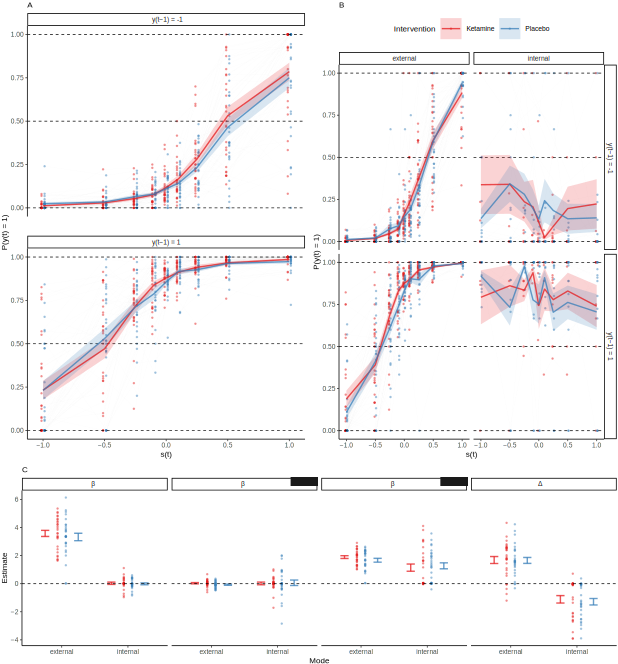
\includegraphics{modes_ketamine_scz_files/figure-latex/rev_Supplemental_Figure_S2-1.pdf}

\textbf{Supplemental Figure S2. Extended data on the effects of
S-ketamine and mode on perceptual inference (related to Figure 2A-C).}

\textbf{A.} Here, we show psychometric curves (percept \(y_t\) versus
input \(s_t\)) under S-ketamine (red) and placebo (blue). The plot
separates times \(t\) for which the previous experience was leftward
rotation (\(y_{t-1} = -1\), upper panel) and rightward rotation
(\(y_{t-1} = +1\), lower panel). As expected, \(y_t\) was driven by both
the external input \(s_t\) (\(\beta_S\) = \(3.01\) ± \(0.06\), z =
\(50.39\), p < \(\ensuremath{2.2\times 10^{-308}}\)) and the previous percept \(y_{t-1}\)
(\(\beta_{P}\) = \(2.06\) ± \(0.03\), z = \(80.58\), p < \(\ensuremath{2.2\times 10^{-308}}\)). We
found no significant interaction between the \(s_t\) and \(y_{t-1}\)
(\(-0.06\) ± \(0.06\), z = \(-1.06\), p = \(1\)). Relative to placebo,
S-ketamine caused a shift of \(y_t\) toward \(s_t\) (\(0.45\) ±
\(0.08\), z = \(5.6\), p = \(\ensuremath{1.71\times 10^{-7}}\)), with no
significant effect on \(y_{t-1}\) (\(0.08\) ± \(0.04\), z = \(2.39\), p
= \(0.13\)). We found no significant three-way-interaction (drug x
\(s_t\) x \(y_{t-1}\), \(-0.07\) ± \(0.08\), z = \(-0.9\), p = \(1\)).

\textbf{B.} This panel shows the data from panel (A) separately for
times \(t\) where the HMM identified the mode of perceptual inference as
external (left panels) or internal (right panels). When the mode of
perceptual processing was added to the prediction of \(y_t\) from
\(s_t\) and \(y_{t-1}\), the effect S-ketamine (red) vs.~placebo (blue)
on \(s_t\) disappeared (\(0.24\) ± \(0.11\), z = \(2.13\), p =
\(0.53\)). Instead, changes in the balance between \(s_t\) and
\(y_{t-1}\) were loaded onto fluctuations between external and internal
mode, which caused perception to shift away from external inputs \(s_t\)
(\(-4.23\) ± \(0.21\), z = \(-20.01\), p =
\(\ensuremath{7.54\times 10^{-88}}\)) and toward previous experiences
\(y{t-1}\) (\(0.78\) ± \(0.09\), z = \(8.64\), p =
\(\ensuremath{8.81\times 10^{-17}}\)).

\textbf{C.} Here, we plot the weights from the GLM
\(y_t = \beta_S \times s_t + \beta_P \times y_{t-1} + \beta_B \times 1\),
alongside the balance between external inputs and previous experiences
\(\Delta_{S-P} = \beta_S - \beta_P\) during external and internal mode.
Colors indicate S-ketamine (red) and placebo (blue). \(\beta_S\), the
weight associated with the external input \(s_t\), was positive in
external mode, but reduced to zero in internal mode (\(-3.55\) ±
\(0.23\), T(\(81\)) = \(-15.44\), p =
\(\ensuremath{4.78\times 10^{-24}}\)). We found no additional effect of
S-ketamine (red) versus placebo (blue; \(-0.25\) ± \(0.23\), T(\(81\)) =
\(-1.1\), p = \(1\)) and no significant interaction (\(0.21\) ±
\(0.33\), T(\(81\)) = \(0.65\), p = \(1\)). \(\beta_B\), the weight
associated with the constant response bias \(b\) toward rightward
rotation, was not different from zero (\(\beta_B\) = \(0.04\) ±
\(0.11\), T(\(98.36\)) = \(0.31\), p = \(1\)). We found no effect of
drug (\(-0.11\) ± \(0.14\), T(\(81\)) = \(-0.74\), p = \(1\)) or mode
(\(-0.02\) ± \(0.14\), T(\(81\)) = \(-0.12\), p = \(1\)) on the bias
weight \(\beta_B\). \(\beta_P\), the weight associated with the previous
percept \(y_{t-1}\) was not modulated by S-ketamine (\(-0.22\) ±
\(0.26\), T(\(81\)) = \(-0.87\), p = \(1\)) or mode (\(-0.75\) ±
\(0.26\), T(\(81\)) = \(-2.92\), p = \(0.29\)). There was no significant
interaction between drug and mode with respect to \(\beta_P\) (\(0.35\)
± \(0.36\), T(\(81\)) = \(0.97\), p = \(1\)). The balance
\(\Delta_{S-P}\) between external inputs and internal predictions was
determined by mode (\(2.8\) ± \(0.29\), T(\(81\)) = \(9.5\), p =
\(\ensuremath{5.22\times 10^{-13}}\)), with no significant effect of
S-ketamine (\(0.03\) ± \(0.29\), T(\(81\)) = \(0.1\), p = \(1\)) and no
interaction (\(0.14\) ± \(0.42\), T(\(81\)) = \(0.34\), p = \(1\)).

\newpage

\hypertarget{supplemental-figure-s3}{%
\subsection{Supplemental Figure S3}\label{supplemental-figure-s3}}

%\includegraphics{modes_ketamine_scz_files/figure-latex/rev_Supplemental_Figure_S3-1.pdf}

\textbf{Supplemental Figure S3. Extended data on external and internal
mode in Scz patients and healthy controls (related to Figure 2E-H).}

\textbf{A.} Here, we show psychometric curves (percept \(y_t\) versus
input \(s_t\)) in patients (red) and controls (blue). The plot separates
times \(t\) for which the previous experience was leftward rotation
(\(y_{t-1} = -1\), upper panel) and rightward rotation
(\(y_{t-1} = +1\), lower panel). Perception was driven by \(s_t\)
(\(\beta_S\) = \(2.77\) ± \(0.11\), z = \(24.85\), p =
\(\ensuremath{2.18\times 10^{-135}}\)) and \(y_{t-1}\) (\(\beta_{P}\) =
\(1.5\) ± \(0.03\), z = \(58.2\), p < \(\ensuremath{2.2\times 10^{-308}}\)), with no significant
interaction between \(s_t\) and \(y_{t-1}\)
(\(\ensuremath{-5.41\times 10^{-3}}\) ± \(0.11\), z = \(-0.05\), p =
\(1\)). Patients were more sensitive to \(s_t\) (\(0.75\) ± \(0.15\), z
= \(4.96\), p = \(\ensuremath{5.6\times 10^{-6}}\)). We found no
significant three-way-interaction (group x \(s_t\) x \(y_{t-1}\),
\(-0.37\) ± \(0.15\), z = \(-2.45\), p = \(0.11\)).

\textbf{B.} This panel shows the data from panel (A) separately for
times \(t\) where the HMM identified the mode of perceptual inference as
external (left panels) or internal (right panels). When the mode of
perceptual processing was added to the prediction of \(y_t\) from
\(s_t\) and \(y_{t-1}\), the difference between patients (red) and
controls (blue) in the effect of \(s_t\) on \(y_t\) disappeared
(\(-0.02\) ± \(0.22\), z = \(-0.08\), p = \(1\)). Instead, changes in
the balance between \(s_t\) and \(y_{t-1}\) were loaded onto
fluctuations between external and internal mode, which caused perception
to shift away from external inputs \(s_t\) (\(-3.47\) ± \(0.29\), z =
\(-11.95\), p = \(\ensuremath{1.01\times 10^{-31}}\)) and toward
previous experiences \(y{t-1}\) (\(0.5\) ± \(0.07\), z = \(6.85\), p =
\(\ensuremath{1.15\times 10^{-10}}\)).

\textbf{C.} Here, we plot the weights from the GLM
\(y_t = \beta_S \times s_t + \beta_P \times y_{t-1} + \beta_B \times 1\),
alongside the balance between external inputs and previous experiences
\(\Delta_{S-P} = \beta_S - \beta_P\) during external and internal mode.
Colors indicate the group (patients in red, controls in blue).
\(\beta_S\), the weight associated with the external input \(s_t\), was
positive in external mode, but reduced to zero in internal mode
(\(-2.19\) ± \(0.24\), T(\(44\)) = \(-9.13\), p =
\(\ensuremath{4.07\times 10^{-11}}\)). We found no additional effect of
group (\(-0.11\) ± \(0.37\), T(\(87.69\)) = \(-0.3\), p = \(1\)) and no
significant interaction (\(-0.25\) ± \(0.34\), T(\(44\)) = \(-0.74\), p
= \(1\)). \(\beta_B\), the weight associated with the constant response
bias \(b\) toward rightward rotation, was not different from zero
(\(0.05\) ± \(0.18\), T(\(\ensuremath{1.62\times 10^{-8}}\)) = \(0.29\),
p = \(1\)). We found no effect of group (\(-0.09\) ± \(0.25\),
T(\(\ensuremath{1.62\times 10^{-8}}\)) = \(-0.37\), p = \(1\)). There
was a trend for a positive effect of internal mode (\(0.6\) ± \(0.24\),
T(\(88\)) = \(2.47\), p = \(0.06\)) on the bias weight \(\beta_B\).
\(\beta_P\), the weight associated with the previous percept
\(y_{t-1}\), was reduced in internal mode (\(-0.75\) ± \(0.26\),
T(\(88\)) = \(-2.92\), p = \(0.02\)), but not modulated by group
(\(0.17\) ± \(0.32\), T(\(\ensuremath{9.88\times 10^{-10}}\)) =
\(0.54\), p = \(1\)). There was no significant interaction between group
and mode with respect to \(\beta_P\) (\(0.11\) ± \(0.36\), T(\(88\)) =
\(0.3\), p = \(1\)). The balance \(\Delta_{S-P}\) between external
inputs and internal predictions was determined by mode (\(1.44\) ±
\(0.33\), T(\(81\)) = \(9.5\), p = \(\ensuremath{3.39\times 10^{-4}}\)),
with no significant effect of group (\(0.28\) ± \(0.54\), T(\(87.97\)) =
\(0.52\), p = \(1\)) and no interaction (\(0.36\) ± \(0.47\), T(\(44\))
= \(0.76\), p = \(1\)).

\newpage

\hypertarget{supplemental-figure-s4}{%
\subsection{Supplemental Figure S4}\label{supplemental-figure-s4}}

%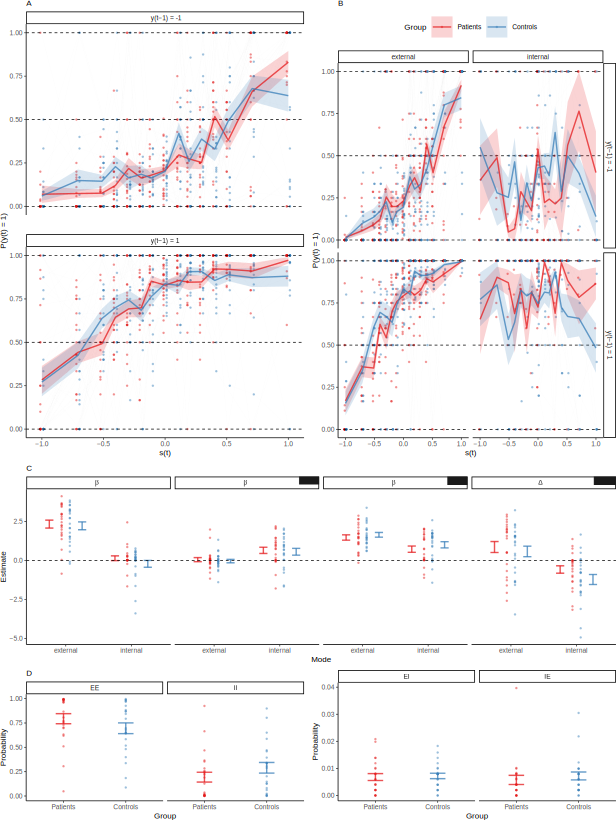
\includegraphics{modes_ketamine_scz_files/figure-latex/rev_Supplemental_Figure_S4-1.pdf}

\textbf{Supplemental Figure S4. RT and bimodal inference in Scz patients
and controls.}

\textbf{A.} RT were non-uniformly distributed across the inter-overlap
interval (D = \(0.22\), p < \(\ensuremath{2.2\times 10^{-308}}\), one-sample Kolmogorov-Smirnov test
against uniformity) in patients (red) and controls (blue). This
confirmed that changes in perception were aligned with the overlapping
configurations of the stimulus.

\textbf{B.} RT did not differ between patients (red) and controls (blue;
\(-0.07\) ± \(0.08\), T(\(66.96\)) = \(-0.87\), p = \(1\)). We found no
quadratic relationship between RT and \(s_t\) (\(-3.54\) ± \(2.34\),
T(\(\ensuremath{5.33\times 10^{3}}\)) = \(-1.51\), p = \(1\)).

\textbf{C.} We found no effect of mode on RT (\(0.03\) ± \(0.04\), z =
\(\ensuremath{4.89\times 10^{3}}\), p = \(0.76\)).

\newpage

\hypertarget{supplemental-figure-s5}{%
\subsection{Supplemental Figure S5}\label{supplemental-figure-s5}}

%\includegraphics{modes_ketamine_scz_files/figure-latex/Supplemental_Figure_S5-1.pdf}

\textbf{Supplemental Figure S5. Scores and Questionnaires.}

\textbf{A.} Responses to Q1 (\emph{How awake do you feel?}) indicated
that participants felt more tired under S-ketamine (red) than placebo
(blue; \(-1.53\) ± \(0.6\), z = \(-2.57\), p = \(0.04\)), with no
significant effect of time or a between-factor interaction. Responses to
Q2 (\emph{How intoxicated do you feel?}) indicated that participants
felt more intoxicated under S-ketamine (\(3.32\) ± \(1.44\), z =
\(2.3\), p = \(0.09\)), with no significant effect of time or a
between-factor interaction. Responses to Q3 (\emph{How nervous do you
feel?}) revealed no effect of S-ketamine (\(-3.01\) ± \(2.62\), z =
\(-1.15\), p = \(1\)), time, nor a significant between-factor
interaction. CADSS scores were elevated under S-ketamine (\(1.01\) ±
\(0.34\), T(\(185.32\)) = \(2.99\), p = \(0.01\)) with a borderline
trend for an increase over time (\(0.09\) ± \(0.04\), T(\(185.61\)) =
\(2.24\), p = \(0.1\)) and no significant between-factor interaction.

\textbf{B.} Q1-3 and CADSS scores were collected after blocks 1, 3, 6
and 9. To assess how the mode of perceptual inference was linked to
dissociative symptoms, we separated the participants ratings according
to the mode that dominated perception at the very end of the preceding
block. While controlling the effect of S-ketamine (red) vs placebo
(blue), we found that external mode increased dissociative symptoms
(\(1.05\) ± \(0.54\), T(\(208.05\)) = \(1.95\), p = \(0.05\)), but had
no effect on wakefulness (Q1), subjective intoxication (Q2) or
nervousness (Q3).

\textbf{C.} 5-ASC scores were elevated under S-ketamine (red) relative
to placebo (blue; \(4.89\) ± \(1.59\), T(\(27.14\)) = \(3.08\), p =
\(\ensuremath{9.33\times 10^{-3}}\)).

\textbf{D.} Neither PDI, CAPS, nor 5-ASC scores were predictive of the
probability of external mode (shown separately for S-ketamine in red and
placebo in blue).

\textbf{E.} Stereodisparity thresholds were not predictive of the
probability of external mode (\(-28.73\) ± \(781.1\), z = \(-0.04\), p =
\(0.97\)). Thresholds did not differ between S-ketamine (red) and
placebo (blue; W = \(102\), p = \(0.66\)).

\textbf{F.} Neither PDI, CAPS (patients in red and controls in blue),
nor the PANSS items P1 (delusions) or P3 (hallucinations, patients only)
predicted the probability of external mode.

\textbf{G.} In patients (red) and controls (blue), stereodisparity
thresholds were not predictive of the probability of external mode
(\(-1.88\) ± \(2.05\), z = \(-0.92\), p = \(1\)). Thresholds did not
differ between groups (V = \(976\), p = \(0.52\)).

\newpage

\hypertarget{supplemental-table-s1}{%
\subsection{Supplemental Table S1}\label{supplemental-table-s1}}

\begin{longtable}[]{@{}
  >{\raggedright\arraybackslash}p{(\columnwidth - 4\tabcolsep) * \real{0.3148}}
  >{\raggedright\arraybackslash}p{(\columnwidth - 4\tabcolsep) * \real{0.4537}}
  >{\raggedright\arraybackslash}p{(\columnwidth - 4\tabcolsep) * \real{0.2315}}@{}}
\toprule\noalign{}
\begin{minipage}[b]{\linewidth}\raggedright
RESOURCE
\end{minipage} & \begin{minipage}[b]{\linewidth}\raggedright
SOURCE
\end{minipage} & \begin{minipage}[b]{\linewidth}\raggedright
IDENTIFIER
\end{minipage} \\
\midrule\noalign{}
\endhead
\bottomrule\noalign{}
\endlastfoot
\textbf{Deposited data \& code} & & \\
Analyzed data \& custom code &
\url{https://github.com/veithweilnhammer/modes_ketamine_scz} & N/A \\
\textbf{Software} & & \\
\textbf{Matlab} & \url{https://www.mathworks.com/} & RRID:SCR\_001622 \\
Psychtoolbox 3 & \url{http://psychtoolbox.org/} & RRID:SCR\_002881 \\
\textbf{R} & \url{http://www.r-project.org/} & RRID:SCR\_001905 \\
RStudio & \url{https://www.rstudio.com/} & RRID:SCR\_000432 \\
lme4, afex, statConfR, ggplot2, ggridges, gridExtra, tidyr, plyr, readxl
& \url{http://cran.r-project.org/} & RRID:SCR\_003005 \\
\textbf{Python 3} & \url{http://www.python.org/} & RRID:SCR\_008394 \\
Jupyter Notebook & \url{https://jupyter.org/} & RRID:SCR\_018315 \\
numpy & \url{http://www.numpy.org} & RRID:SCR\_008633 \\
pandas & \url{https://pandas.pydata.org} & RRID:SCR\_018214 \\
SSM & \url{https://github.com/lindermanlab/ssm} & N/A \\
\end{longtable}

\textbf{Supplemental Table S1. Key resources.}

\newpage

\hypertarget{supplemental-table-s2}{%
\subsection{Supplemental Table S2}\label{supplemental-table-s2}}

\begin{longtable}[]{@{}
  >{\raggedright\arraybackslash}p{(\columnwidth - 6\tabcolsep) * \real{0.1818}}
  >{\raggedright\arraybackslash}p{(\columnwidth - 6\tabcolsep) * \real{0.4364}}
  >{\raggedright\arraybackslash}p{(\columnwidth - 6\tabcolsep) * \real{0.1818}}
  >{\raggedright\arraybackslash}p{(\columnwidth - 6\tabcolsep) * \real{0.2000}}@{}}
\toprule\noalign{}
\begin{minipage}[b]{\linewidth}\raggedright
Scale
\end{minipage} & \begin{minipage}[b]{\linewidth}\raggedright
Scope
\end{minipage} & \begin{minipage}[b]{\linewidth}\raggedright
Condition
\end{minipage} & \begin{minipage}[b]{\linewidth}\raggedright
mean ± s.e.m.
\end{minipage} \\
\midrule\noalign{}
\endhead
\bottomrule\noalign{}
\endlastfoot
\textbf{PDI}\textsuperscript{27} & Delusion proneness & Global & 46.22 ±
7.19 \\
\textbf{CAPS}\textsuperscript{28} & Hallucination proneness & Global &
23 ± 5.05 \\
\textbf{BPRS}\textsuperscript{29} & Screen for psychotic illness &
Global & 0.64 ± 0.27 \\
\textbf{5D-ASC}\textsuperscript{31} & Altered states of consciousness &
S-ketamine & 7.11 ± 1.59 \\
& & Placebo & 2.2 ± 0.75 \\
\textbf{CADSS}\textsuperscript{23} & Dissociation & S-ketamine & 7.8 ±
0.33 \\
& & Placebo & 6.43 ± 0.17 \\
\textbf{Q1} & Wakefulness & S-ketamine & 0.41 ± 0.03 \\
& & Placebo & 0.48 ± 0.03 \\
\textbf{Q2} & Intoxication & S-ketamine & 0.29 ± 0.03 \\
& & Placebo & 0.09 ± 0.02 \\
\textbf{Q3} & Nervousness & S-ketamine & 0.17 ± 0.02 \\
& & Placebo & 0.13 ± 0.03 \\
\textbf{Stereovision} & Disparity thresholds & S-ketamine &
\ensuremath{2.89\times 10^{-3}} ± \ensuremath{6.18\times 10^{-4}} \\
& & Placebo & \ensuremath{2.75\times 10^{-3}} ±
\ensuremath{4.39\times 10^{-4}} \\
\end{longtable}

\textbf{Supplemental Table S2. Psychometric data for the S-ketamine
experiment.}

\newpage

\hypertarget{supplemental-table-s3}{%
\subsection{Supplemental Table S3}\label{supplemental-table-s3}}

\begin{longtable}[]{@{}
  >{\raggedright\arraybackslash}p{(\columnwidth - 6\tabcolsep) * \real{0.1818}}
  >{\raggedright\arraybackslash}p{(\columnwidth - 6\tabcolsep) * \real{0.4364}}
  >{\raggedright\arraybackslash}p{(\columnwidth - 6\tabcolsep) * \real{0.1818}}
  >{\raggedright\arraybackslash}p{(\columnwidth - 6\tabcolsep) * \real{0.2000}}@{}}
\toprule\noalign{}
\begin{minipage}[b]{\linewidth}\raggedright
Scale
\end{minipage} & \begin{minipage}[b]{\linewidth}\raggedright
Scope
\end{minipage} & \begin{minipage}[b]{\linewidth}\raggedright
Condition
\end{minipage} & \begin{minipage}[b]{\linewidth}\raggedright
mean ± s.e.m.
\end{minipage} \\
\midrule\noalign{}
\endhead
\bottomrule\noalign{}
\endlastfoot
\textbf{PDI}\textsuperscript{27} & Delusion proneness & Patients &
138.83 ± 16.64 \\
& & Controls & 21.87 ± 5.75 \\
\textbf{CAPS}\textsuperscript{28} & Hallucination proneness & Patients &
65.17 ± 10.56 \\
& & Controls & 7.13 ± 2.2 \\
\textbf{P1} & Delusions & Patients & 3.83 ± 0.39 \\
\textbf{P3} & Delusions & Patients & 3.35 ± 0.44 \\
\textbf{Stereovision} & Disparity thresholds & Patients &
\ensuremath{2.82\times 10^{-3}} ± \ensuremath{5.13\times 10^{-4}} \\
& & Controls & \ensuremath{3.46\times 10^{-3}} ±
\ensuremath{7.14\times 10^{-4}} \\
\end{longtable}

\textbf{Supplemental Table S3. Psychometric data for Scz-control-study.}

\newpage

\hypertarget{references}{%
\section*{References}\label{references}}
\addcontentsline{toc}{section}{References}

\hypertarget{refs}{}
\begin{CSLReferences}{0}{0}
\leavevmode\vadjust pre{\hypertarget{ref-fletcher_perceiving_2009}{}}%
\CSLLeftMargin{1. }%
\CSLRightInline{Fletcher, P. C. \emph{et al.}
\href{https://doi.org/10.1038/nrn2536}{Perceiving is believing: A
{Bayesian} approach to explaining the positive symptoms of
schizophrenia}. \emph{Nature Reviews Neuroscience} \textbf{10}, 48--58
(2009).}

\leavevmode\vadjust pre{\hypertarget{ref-Adams2013}{}}%
\CSLLeftMargin{2. }%
\CSLRightInline{Adams, R. A. \emph{et al.}
\href{https://doi.org/10.3389/fpsyt.2013.00047}{The computational
anatomy of psychosis.} \emph{Frontiers in psychiatry} \textbf{4}, 47
(2013).}

\leavevmode\vadjust pre{\hypertarget{ref-Sterzer2018}{}}%
\CSLLeftMargin{3. }%
\CSLRightInline{Sterzer, P. \emph{et al.}
\href{https://doi.org/10.1016/j.biopsych.2018.05.015}{The {Predictive}
{Coding} {Account} of {Psychosis}}. \emph{Biological Psychiatry}
\textbf{84}, 634--643 (2018).}

\leavevmode\vadjust pre{\hypertarget{ref-corlett_glutamatergic_2011}{}}%
\CSLLeftMargin{4. }%
\CSLRightInline{Corlett, P. R. \emph{et al.}
\href{https://doi.org/10.1038/npp.2010.163}{Glutamatergic {Model}
{Psychoses}: {Prediction} {Error}, {Learning}, and {Inference}}.
\emph{Neuropsychopharmacology} \textbf{36}, 294--315 (2011).}

\leavevmode\vadjust pre{\hypertarget{ref-Stein2020}{}}%
\CSLLeftMargin{5. }%
\CSLRightInline{Stein, H. \emph{et al.}
\href{https://doi.org/10.1038/s41467-020-18033-3}{Reduced serial
dependence suggests deficits in synaptic potentiation in anti-{NMDAR}
encephalitis and schizophrenia}. \emph{Nature Communications}
\textbf{11}, 1--11 (2020).}

\leavevmode\vadjust pre{\hypertarget{ref-murray_linking_2014}{}}%
\CSLLeftMargin{6. }%
\CSLRightInline{Murray, J. D. \emph{et al.}
\href{https://doi.org/10.1093/cercor/bhs370}{Linking {Microcircuit}
{Dysfunction} to {Cognitive} {Impairment}: {Effects} of {Disinhibition}
{Associated} with {Schizophrenia} in a {Cortical} {Working} {Memory}
{Model}}. \emph{Cerebral Cortex} \textbf{24}, 859--872 (2014).}

\leavevmode\vadjust pre{\hypertarget{ref-catts_quantitative_2016}{}}%
\CSLLeftMargin{7. }%
\CSLRightInline{Catts, V. S. \emph{et al.}
\href{https://doi.org/10.1016/j.biopsycho.2015.10.013}{A quantitative
review of the postmortem evidence for decreased cortical
{N}-methyl-{D}-aspartate receptor expression levels in schizophrenia:
{How} can we link molecular abnormalities to mismatch negativity
deficits?} \emph{Biological Psychology} \textbf{116}, 57--67 (2016).}

\leavevmode\vadjust pre{\hypertarget{ref-wang_nmda_2013}{}}%
\CSLLeftMargin{8. }%
\CSLRightInline{Wang, M. \emph{et al.}
\href{https://doi.org/10.1016/j.neuron.2012.12.032}{{NMDA} {Receptors}
{Subserve} {Persistent} {Neuronal} {Firing} during {Working} {Memory} in
{Dorsolateral} {Prefrontal} {Cortex}}. \emph{Neuron} \textbf{77},
736--749 (2013).}

\leavevmode\vadjust pre{\hypertarget{ref-nakao_schizophrenia-like_2019}{}}%
\CSLLeftMargin{9. }%
\CSLRightInline{Nakao, K. \emph{et al.}
\href{https://doi.org/10.1093/schbul/sby003}{Schizophrenia-{Like}
{Dopamine} {Release} {Abnormalities} in a {Mouse} {Model} of {NMDA}
{Receptor} {Hypofunction}}. \emph{Schizophrenia Bulletin} \textbf{45},
138--147 (2019).}

\leavevmode\vadjust pre{\hypertarget{ref-self_different_2012}{}}%
\CSLLeftMargin{10. }%
\CSLRightInline{Self, M. W. \emph{et al.}
\href{https://doi.org/10.1073/pnas.1119527109}{Different glutamate
receptors convey feedforward and recurrent processing in macaque {V1}}.
\emph{Proceedings of the National Academy of Sciences} \textbf{109},
11031--11036 (2012).}

\leavevmode\vadjust pre{\hypertarget{ref-castro-alamancos_short-term_1996}{}}%
\CSLLeftMargin{11. }%
\CSLRightInline{Castro-Alamancos, M. A. \emph{et al.}
\href{https://doi.org/10.1073/pnas.93.3.1335}{Short-term synaptic
enhancement and long-term potentiation in neocortex.} \emph{Proceedings
of the National Academy of Sciences} \textbf{93}, 1335--1339 (1996).}

\leavevmode\vadjust pre{\hypertarget{ref-oorschot_temporal_2012}{}}%
\CSLLeftMargin{12. }%
\CSLRightInline{Oorschot, M. \emph{et al.}
\href{https://doi.org/10.1016/j.schres.2012.06.010}{Temporal dynamics of
visual and auditory hallucinations in psychosis}. \emph{Schizophrenia
Research} \textbf{140}, 77--82 (2012).}

\leavevmode\vadjust pre{\hypertarget{ref-hermans_temporal_2020}{}}%
\CSLLeftMargin{13. }%
\CSLRightInline{Hermans, K. \emph{et al.}
\href{https://doi.org/10.1016/j.psychres.2020.113039}{Temporal dynamics
of suspiciousness and hallucinations in clinical high risk and first
episode psychosis}. \emph{Psychiatry Research} \textbf{290}, 113039
(2020).}

\leavevmode\vadjust pre{\hypertarget{ref-laquitaine_switching_2018}{}}%
\CSLLeftMargin{14. }%
\CSLRightInline{Laquitaine, S. \emph{et al.}
\href{https://doi.org/10.1016/j.neuron.2017.12.011}{A {Switching}
{Observer} for {Human} {Perceptual} {Estimation}}. \emph{Neuron}
\textbf{97}, 462--474.e6 (2018).}

\leavevmode\vadjust pre{\hypertarget{ref-roy_extracting_2021}{}}%
\CSLLeftMargin{15. }%
\CSLRightInline{Roy, N. A. \emph{et al.}
\href{https://doi.org/10.1016/J.NEURON.2020.12.004}{Extracting the
dynamics of behavior in sensory decision-making experiments}.
\emph{Neuron} \textbf{109}, 597--610.e6 (2021).}

\leavevmode\vadjust pre{\hypertarget{ref-ashwood_mice_2022}{}}%
\CSLLeftMargin{16. }%
\CSLRightInline{Ashwood, Z. C. \emph{et al.}
\href{https://doi.org/10.1038/s41593-021-01007-z}{Mice alternate between
discrete strategies during perceptual decision-making}. \emph{Nature
Neuroscience} \textbf{25}, 201--212 (2022).}

\leavevmode\vadjust pre{\hypertarget{ref-weilnhammer_sensory_2023}{}}%
\CSLLeftMargin{17. }%
\CSLRightInline{Weilnhammer, V. \emph{et al.}
\href{https://doi.org/10.1371/journal.pbio.3002410}{Sensory processing
in humans and mice fluctuates between external and internal modes}.
\emph{PLOS Biology} \textbf{21}, e3002410 (2023).}

\leavevmode\vadjust pre{\hypertarget{ref-albert_hierarchical_2017}{}}%
\CSLLeftMargin{18. }%
\CSLRightInline{Albert, S. \emph{et al.}
\href{https://doi.org/10.1371/journal.pcbi.1005856}{A hierarchical
stochastic model for bistable perception}. \emph{PLOS Computational
Biology} \textbf{13}, e1005856 (2017).}

\leavevmode\vadjust pre{\hypertarget{ref-weilnhammer_psychotic_2020}{}}%
\CSLLeftMargin{19. }%
\CSLRightInline{Weilnhammer, V. \emph{et al.}
\href{http://www.ncbi.nlm.nih.gov/pubmed/32090246}{Psychotic
{Experiences} in {Schizophrenia} and {Sensitivity} to {Sensory}
{Evidence}.} \emph{Schizophrenia bulletin} \textbf{46}, 927--936
(2020).}

\leavevmode\vadjust pre{\hypertarget{ref-weilnhammer_active_2021}{}}%
\CSLLeftMargin{20. }%
\CSLRightInline{Weilnhammer, V. \emph{et al.}
\href{https://doi.org/10.1016/j.cub.2021.04.043}{An active role of
inferior frontal cortex in conscious experience}. \emph{Current Biology}
\textbf{31}, 2868--2880.e8 (2021).}

\leavevmode\vadjust pre{\hypertarget{ref-muckli_contextual_2015}{}}%
\CSLLeftMargin{21. }%
\CSLRightInline{Muckli, L. \emph{et al.}
\href{https://doi.org/10.1016/j.cub.2015.08.057}{Contextual {Feedback}
to {Superficial} {Layers} of {V1}}. \emph{Current Biology} \textbf{25},
2690--2695 (2015).}

\leavevmode\vadjust pre{\hypertarget{ref-weilnhammer_neural_2018}{}}%
\CSLLeftMargin{22. }%
\CSLRightInline{Weilnhammer, V. \emph{et al.}
\href{https://doi.org/10.1523/JNEUROSCI.2901-17.2018}{The {Neural}
{Correlates} of {Hierarchical} {Predictions} for {Perceptual}
{Decisions}}. \emph{The Journal of Neuroscience} \textbf{38}, 5008--5021
(2018).}

\leavevmode\vadjust pre{\hypertarget{ref-mertens_clinician-administered_2022}{}}%
\CSLLeftMargin{23. }%
\CSLRightInline{Mertens, Y. L. \emph{et al.}
\href{https://doi.org/10.1080/15299732.2021.1989111}{The
{Clinician}-{Administered} {Dissociative} {States} {Scale} ({CADSS}):
{Validation} of the {German} {Version}}. \emph{Journal of Trauma \&
Dissociation} \textbf{23}, 366--384 (2022).}

\leavevmode\vadjust pre{\hypertarget{ref-schmack_striatal_2021}{}}%
\CSLLeftMargin{24. }%
\CSLRightInline{Schmack, K. \emph{et al.}
\href{https://doi.org/10.1126/science.abf4740}{Striatal dopamine
mediates hallucination-like perception in mice}. \emph{Science (New
York, N.Y.)} \textbf{372}, eabf4740 (2021).}

\leavevmode\vadjust pre{\hypertarget{ref-longden_relationship_2020}{}}%
\CSLLeftMargin{25. }%
\CSLRightInline{Longden, E. \emph{et al.}
\href{https://doi.org/10.1093/schbul/sbaa037}{The {Relationship}
{Between} {Dissociation} and {Symptoms} of {Psychosis}: {A}
{Meta}-analysis}. \emph{Schizophrenia Bulletin} \textbf{46}, 1104--1113
(2020).}

\leavevmode\vadjust pre{\hypertarget{ref-harrison_grin2a_2023}{}}%
\CSLLeftMargin{26. }%
\CSLRightInline{Harrison, P. J. \emph{et al.}
\href{https://doi.org/10.1038/s41380-023-02265-y}{{GRIN2A} ({NR2A}): A
gene contributing to glutamatergic involvement in schizophrenia}.
\emph{Molecular Psychiatry} \textbf{28}, 3568--3572 (2023).}

\leavevmode\vadjust pre{\hypertarget{ref-Peters1999}{}}%
\CSLLeftMargin{27. }%
\CSLRightInline{Peters, E. R. \emph{et al.}
\href{https://www.ncbi.nlm.nih.gov/pubmed/10478789}{Measurement of
delusional ideation in the normal population: Introducing the {PDI}
({Peters} et al. {Delusions} {Inventory}).} \emph{Schizophrenia
bulletin} \textbf{25}, 553--76 (1999).}

\leavevmode\vadjust pre{\hypertarget{ref-Bell2006}{}}%
\CSLLeftMargin{28. }%
\CSLRightInline{Bell, V. \emph{et al.}
\href{https://doi.org/10.1093/schbul/sbj014}{The {Cardiff} {Anomalous}
{Perceptions} {Scale} ({CAPS}): {A} {New} {Validated} {Measure} of
{Anomalous} {Perceptual} {Experience}}. \emph{Schizophrenia Bulletin}
\textbf{32}, 366--377 (2006).}

\leavevmode\vadjust pre{\hypertarget{ref-overall_brief_1962}{}}%
\CSLLeftMargin{29. }%
\CSLRightInline{Overall, J. E. \emph{et al.}
\href{https://doi.org/10.2466/pr0.1962.10.3.799}{The {Brief}
{Psychiatric} {Rating} {Scale}}. \emph{Psychological Reports}
\textbf{10}, 799--812 (1962).}

\leavevmode\vadjust pre{\hypertarget{ref-Brainard1997}{}}%
\CSLLeftMargin{30. }%
\CSLRightInline{Brainard, D. H.
\href{https://www.ncbi.nlm.nih.gov/pubmed/9176952}{The {Psychophysics}
{Toolbox}.} \emph{Spatial vision} \textbf{10}, 433--6 (1997).}

\leavevmode\vadjust pre{\hypertarget{ref-dittrich_5d-abz_1999}{}}%
\CSLLeftMargin{31. }%
\CSLRightInline{Dittrich, A. \emph{et al.} {5D}-{ABZ}: {Fragebogen} zur
{Erfassung} {Aussergewöhnlicher} {Bewusstseinszustände}. \emph{Eine
kurze Einführung. PSIN Plus, Zürich} (1999).}

\leavevmode\vadjust pre{\hypertarget{ref-Kay1987}{}}%
\CSLLeftMargin{32. }%
\CSLRightInline{Kay, S. R. \emph{et al.}
\href{https://www.ncbi.nlm.nih.gov/pubmed/3616518}{The positive and
negative syndrome scale ({PANSS}) for schizophrenia.}
\emph{Schizophrenia bulletin} \textbf{13}, 261--76 (1987).}

\leavevmode\vadjust pre{\hypertarget{ref-linderman_ssm_2020}{}}%
\CSLLeftMargin{33. }%
\CSLRightInline{Linderman, S. \emph{et al.}
\href{https://github.com/lindermanlab/ssm}{{SSM}: {Bayesian} {Learning}
and {Inference} for {State} {Space} {Models}}. (2020).}

\end{CSLReferences}

\end{document}
